\documentclass[10pt,a4paper]{article}

\usepackage[utf8]{inputenc}
\usepackage[T1]{fontenc}
\usepackage[english,italian]{babel}
\usepackage{lmodern}
\usepackage{textcomp}
\usepackage{microtype}
\usepackage[a4paper,margin=2.15cm,headheight=14pt]{geometry}
\usepackage{graphicx}
\usepackage{booktabs}
\usepackage{array}
\usepackage{longtable}
\usepackage{amsmath,amssymb}
\usepackage{xcolor}
\usepackage{hyperref}
\usepackage{xurl}
\usepackage{natbib}
\usepackage{caption}
\usepackage{float}
\usepackage{pdflscape}
\usepackage{fancyhdr}
\usepackage{enumitem}

\definecolor{dvnsblue}{HTML}{155EEF}
\definecolor{dvnsnavy}{HTML}{16324F}
\definecolor{dvnsteal}{HTML}{087E8B}
\definecolor{dvnsgreen}{HTML}{228B5B}
\definecolor{dvnsamber}{HTML}{D97706}
\definecolor{dvnsgrey}{HTML}{667085}
\definecolor{dvnslight}{HTML}{E8EEF5}

\hypersetup{
  colorlinks=true,
  linkcolor=dvnsnavy,
  citecolor=dvnsteal,
  urlcolor=dvnsblue,
  pdftitle={Dai fondi ai posti: l'equita territoriale alla prova dell'esecuzione dei progetti PNRR per gli asili nido},
  pdfauthor={DoveVannoINostriSoldi}
}

\graphicspath{{../figures/}}
\captionsetup{font=small,labelfont=bf}
\setlength{\parindent}{0pt}
\setlength{\parskip}{5pt plus 1pt}
\setlist[itemize]{leftmargin=1.4em,itemsep=2pt,topsep=3pt}
\setlist[enumerate]{leftmargin=1.5em,itemsep=3pt,topsep=3pt}
\renewcommand{\arraystretch}{1.12}

\pagestyle{fancy}
\fancyhf{}
\fancyhead[L]{\small\color{dvnsgrey}Dai fondi ai posti}
\fancyhead[R]{\small\color{dvnsgrey}DoveVannoINostriSoldi}
\fancyfoot[C]{\thepage}

\newcommand{\keybox}[1]{%
  \begin{center}
  \fcolorbox{dvnsteal}{dvnslight}{\parbox{0.91\textwidth}{#1}}
  \end{center}
}
\newcommand{\euro}{\,€}

\begin{document}

\begin{titlepage}
  \thispagestyle{empty}
  \vspace*{1.7cm}
  {\color{dvnsblue}\rule{\textwidth}{3pt}}\\[1.1cm]
  {\Huge\bfseries\color{dvnsnavy} Dai fondi ai posti\par}
  \vspace{0.45cm}
  {\LARGE L'equità territoriale alla prova dell'esecuzione dei progetti PNRR per gli asili nido\par}
  \vspace{0.65cm}
  {\large Avanzamento amministrativo, struttura degli appalti e limiti della verificabilità pubblica\par}
  \vfill
  {\large\bfseries DoveVannoINostriSoldi\par}
  {\normalsize Laboratorio di ricerca civica sui conti pubblici\par}
  \vspace{0.5cm}
  {\normalsize 29 agosto 2026 -- Working paper 1.0\par}
  \vfill
  \keybox{\textbf{Confine interpretativo.} Questo studio misura lo stato amministrativo dei progetti, non i posti effettivamente aperti o certificati. I dati pubblici analizzati non contengono il numero di posti creati per CUP né il relativo certificato di completamento.}
  \vspace{0.4cm}
  {\small\color{dvnsgrey}Dati di attuazione Italia Domani, integrati e verificati tramite l'MCP di DoveVannoINostriSoldi; statistiche territoriali Istat. Codice, tabelle, hash e artefatti di riproduzione accompagnano il paper.\par}
  \vspace{0.8cm}
  {\color{dvnsblue}\rule{\textwidth}{1pt}}
\end{titlepage}

\section*{Sintesi esecutiva}

Il target europeo M4C1-18 richiede certificati di completamento per almeno 150.480 posti nei servizi educativi 0--6 entro il secondo trimestre 2026 \citep{ec2026target}. A diciassette giorni dalla fine del trimestre, lo snapshot pubblico del 13 giugno 2026 permette di osservare progetti, fasi, finanziamenti e gare, ma non il numero di posti certificati. Il paper risponde quindi a una domanda più circoscritta e verificabile: \emph{quali progetti classificati come asili nido hanno raggiunto la conclusione amministrativa o almeno il collaudo, e dove si concentra il rischio di esecuzione?}

I risultati principali sono cinque.

\begin{enumerate}
  \item \textbf{Solo 294 progetti su 2.980 risultano conclusi (9,9\%).} Altri 1.149 sono in collaudo ma non conclusi; 1.371 sono ancora in esecuzione lavori. La metà amministrativamente più matura della pipeline non equivale alla metà dei posti certificati: il denominatore richiesto dall'Unione europea non è osservabile.
  \item \textbf{L'investimento sembra redistributivo, l'esecuzione molto meno.} A livello regionale il finanziamento associato per bambino 0--2 è più elevato dove la copertura preesistente era più bassa (correlazione di Spearman $\rho=-0{,}58$), ma la quota di progetti conclusi o in collaudo cresce con la copertura preesistente ($\rho=0{,}59$). È una tensione tra equità di allocazione ed equità di realizzazione, non una stima causale.
  \item \textbf{Il tempo conta più della retorica sulle gare.} A parità delle altre variabili osservate, un anno di avvio più recente è associato a odds di conclusione circa dimezzate (OR 0,47) e a odds di aver raggiunto il collaudo inferiori del 37\% (OR 0,63). Un raddoppio del finanziamento è anch'esso associato a minore maturità. Ampliamenti e ristrutturazioni risultano più avanzati delle nuove costruzioni.
  \item \textbf{Il numero di procedure è una traccia, non una cura.} Il 94,5\% dei progetti ha almeno una procedura; una gara lavori compare nel 94--98\% dei progetti in esecuzione, collaudo o conclusi. Controllando per scala, tipo e anno di avvio, il raddoppio del numero di procedure ha un'associazione piccola e non sempre statisticamente distinguibile da zero. Non emerge evidenza che “riformare la gara” basti a spiegare la fase di consegna.
  \item \textbf{Il vero collo di bottiglia informativo è l'esito.} Regione, finanziamento e importi di gara sono quasi completi; la data di aggiudicazione è presente nel 69,6\% delle procedure. Mancano invece un registro pubblico CUP--posti, i certificati di completamento, la data storica dei passaggi di fase e misure di apertura, personale e utilizzo del servizio.
\end{enumerate}

La conclusione di policy è operativa: la priorità non è un altro contatore aggregato. Serve un registro di consegna che colleghi ogni CUP ai posti previsti, completati, certificati e realmente attivati, preservando lo storico delle revisioni. Senza questa infrastruttura, l'amministrazione può dimostrare l'avanzamento procedurale ma la società non può verificare in modo indipendente il risultato pubblico.

\clearpage
\tableofcontents
\clearpage

\section*{Abstract}
\addcontentsline{toc}{section}{Abstract}

Questo studio analizza l'avanzamento amministrativo di 2.980 progetti classificati come \emph{asili nido} nella misura PNRR M4C1I1.1, utilizzando microdati Italia Domani con riferimento 13 giugno 2026, integrati tramite l'infrastruttura DoveVannoINostriSoldi. Costruiamo due esiti osservabili --- conclusione amministrativa e raggiungimento almeno del collaudo --- e li colleghiamo a tipo di opera, scala finanziaria, anno di avvio, impronta degli appalti e copertura regionale dei servizi 0--2 rilevata da Istat. Il 9,9\% dei progetti risulta concluso e il 48,4\% almeno in collaudo. La copertura preesistente è positivamente associata alla maturità, mentre il finanziamento per bambino è maggiore nelle regioni a minore copertura. Regressioni logistiche con errori standard raggruppati per regione mostrano associazioni robuste tra maggiore maturità, avvio anticipato, minore scala finanziaria e interventi di ampliamento o recupero rispetto alle nuove costruzioni. Il paper non stima effetti causali e non misura il conseguimento del target europeo, perché i dati aperti non pubblicano posti creati e certificati per CUP. Il contributo è duplice: una fotografia riproducibile della pipeline alla vigilia della scadenza e una specifica minima dei dati necessari per passare dal monitoraggio della spesa alla verifica del servizio.

\textbf{Parole chiave:} PNRR; asili nido; capacità amministrativa; appalti pubblici; equità territoriale; open data.\\
\textbf{Codici JEL:} H54, H75, I28, R58.

\begin{otherlanguage}{english}
\section*{Abstract in English}
This paper studies the administrative maturity of 2,980 projects explicitly classified as nursery facilities under Italy's NRRP measure M4C1I1.1. We use project-level Italy Tomorrow data as of 13 June 2026, integrated through the DoveVannoINostriSoldi infrastructure, and define two observable outcomes: recorded administrative completion and having reached at least the commissioning stage. Only 9.9 percent of projects are recorded as completed and 48.4 percent as completed or under commissioning. Regional baseline childcare coverage is positively associated with maturity, while funding per estimated child is higher in low-coverage regions. Logistic models with region-clustered standard errors associate earlier starts, smaller financial scale, and expansion or renovation projects with greater maturity than new construction. The analysis is descriptive, not causal. Crucially, it cannot assess the EU target because open project data do not report completed and certified places by project. We contribute a reproducible near-deadline assessment of the delivery pipeline and a minimum data specification for moving from expenditure monitoring to outcome verification.
\end{otherlanguage}

\section{Perché studiare l'esecuzione, non solo l'allocazione}

L'espansione dei servizi per la prima infanzia è una politica del lavoro, dell'istruzione e dell'equità territoriale. Per l'Italia, l'evidenza sulla maggiore disponibilità di servizi sovvenzionati indica effetti rilevanti sulla partecipazione e sull'occupazione materna, senza peggioramenti osservati negli esiti cognitivi studiati \citep{carta2018}. La rilevanza sociale dell'investimento non garantisce però la sua consegna. La governance dei servizi combina responsabilità nazionali e locali, infrastrutture e spesa corrente, standard comuni e capacità amministrative diseguali \citep{lippi2023,torrini2025}.

Il PNRR ha reso questa tensione misurabile. Nell'allegato della Commissione del marzo 2026, il target M4C1-18 resta definito come certificati di completamento per almeno 150.480 posti nuovi, riqualificati, ampliati o derivanti da cambio d'uso nei servizi 0--6, con al massimo 35.000 posti da demolizione e ricostruzione \citep{ec2026target}. L'unità del target è dunque il \emph{posto certificato}, non l'euro assegnato, il progetto finanziato o la gara aggiudicata.

L'ultimo approfondimento istituzionale microterritoriale disponibile prima della nostra finestra, il Focus UPB con dati ReGiS al 9 dicembre 2024, documentava difficoltà di adesione, ritardi di spesa, una quota molto bassa di progetti conclusi e un possibile scarto conservativo di circa 17.400 posti \citep{upb2025}. Studi successivi hanno approfondito la distribuzione spaziale attesa e la possibilità di correggere la mancata copertura mediante mobilità intercomunale \citep{zanardi2026}. Rimaneva aperta una domanda diversa: come appare la \emph{pipeline di consegna} immediatamente prima della scadenza?

\subsection{Domanda di ricerca e contributo}

La domanda principale è:

\begin{quote}
\emph{A diciassette giorni dalla fine del secondo trimestre 2026, quali caratteristiche distinguono i progetti per asili nido amministrativamente conclusi o giunti al collaudo da quelli ancora in esecuzione o in fasi precedenti?}
\end{quote}

Il contributo è deliberatamente circoscritto.

\begin{itemize}
  \item aggiorna la fotografia dei progetti con una data di riferimento prossima alla scadenza;
  \item separa la maturità amministrativa dal conseguimento del target fisico;
  \item collega la pipeline a tipologia, scala e cronologia del progetto, nonché alla sua impronta di procurement;
  \item confronta bisogno territoriale preesistente, intensità finanziaria e avanzamento;
  \item rende ogni trasformazione riproducibile con manifest MCP, hash, codice e tabelle generate.
\end{itemize}

Non valutiamo l'impatto dei nidi su occupazione, natalità o sviluppo dei bambini. Non stimiamo l'effetto causale della capacità amministrativa. Non prevediamo quanti posti saranno certificati. Il paper individua ciò che i dati consentono di osservare e, con pari importanza, ciò che non consentono di concludere.

\section{Contesto: bisogno, capacità e rischio di consegna}

Nell'anno educativo 2023/24 Istat censisce 14.570 servizi e 378.496 posti autorizzati, pari a 31,6 posti ogni 100 bambini 0--2. La media nasconde una geografia netta: il Centro raggiunge il 40,4\%, il Nord-est il 39,1\%, mentre Sud e Isole si fermano rispettivamente al 19,0\% e al 19,5\%. Anche l'incremento recente è stato trainato soprattutto dal privato: il 78,4\% dei circa 12.500 posti aggiuntivi rispetto all'anno precedente \citep{istat2026}.

La distribuzione del bisogno è una parte della politica; la capacità di trasformare risorse in opere è l'altra. La letteratura italiana trova che qualità burocratica, capacità amministrativa e caratteristiche del comune sono associate ai tempi di spesa e di realizzazione \citep{delmonte2025,cerqua2025}. Più in generale, l'OCSE individua competenze, coordinamento e misure di performance come condizioni necessarie per l'efficacia del settore pubblico italiano \citep{bulman2021}. Queste evidenze motivano l'analisi, ma non autorizzano a usare regione o numero di gare come sostituti diretti della capacità amministrativa.

Formuliamo quattro attese descrittive:

\begin{enumerate}
  \item progetti avviati prima dovrebbero trovarsi in fasi più mature;
  \item nuove costruzioni e progetti più grandi potrebbero richiedere tempi più lunghi di ampliamenti e recuperi;
  \item territori con minore copertura potrebbero ricevere più risorse per bambino, ma non necessariamente consegnarle allo stesso ritmo;
  \item il numero e il tipo di procedure dovrebbero essere letti come impronta del ciclo progettuale, non come trattamento esogeno.
\end{enumerate}

\section{Dati e costruzione del campione}

\subsection{Fonti di progetto e verifica MCP}

La fonte primaria è il catalogo open data Italia Domani, licenza CC BY 4.0 \citep{italiadomani2026}. DoveVannoINostriSoldi integra quattro asset ufficiali:

\begin{itemize}
  \item progetti PNRR, da cui provengono CUP, classificazione, stato, cronologia e finanziamenti;
  \item gare, collegate per CUP e identificativi CIG/PDA;
  \item localizzazioni, collegate per CUP;
  \item aggiudicatari, usati solo per controllare la copertura dei collegamenti e mai nell'analisi dei soggetti.
\end{itemize}

La query MCP \texttt{pnrr\_asili} restituisce 3.841 progetti, 18.851 procedure, 3.842 localizzazioni e 18.250 righe aggiudicatario, con data di riferimento 13 giugno 2026 \citep{dvns2026}. Lo snapshot locale è accettato dall'analisi solo se hash, numerosità e totale finanziario coincidono con il manifest interrogato sull'endpoint di produzione. Gli hash completi sono riportati nell'Appendice~\ref{app:repro}.

\subsection{Perché il campione principale contiene 2.980 progetti}

L'intera misura riguarda servizi 0--6. Il benchmark Istat disponibile e comparabile misura invece i posti per bambini 0--2. Per evitare di associare la copertura dei nidi a interventi per scuole materne, il campione principale include solo i 2.980 record la cui categoria ufficiale è \texttt{ASILI NIDO}. Essi rappresentano il 77,6\% dei progetti della misura e 3,29 miliardi di euro di finanziamento totale associato. I 3.841 progetti 0--6 restano nel controllo di robustezza.

Questa scelta privilegia la validità del confronto territoriale. Non implica che ogni record classificato come nido produca esclusivamente posti 0--2, né che le altre categorie siano estranee alla politica per l'infanzia. È un filtro amministrativo riproducibile, non una riclassificazione sostanziale delle opere.

\begin{table}[H]
\centering
\caption{Campione e grandezze principali}
\label{tab:summary}
\resizebox{\textwidth}{!}{\begin{tabular}{lrl}
\toprule
Indicatore & Valore & Unità/nota \\
\midrule
Campione principale: asili nido & 2.980 & progetti \\
Intera misura M4C1-18 & 3.841 & controllo 0--6 anni \\
Comuni interessati & 2.307 & codici ISTAT composti \\
Finanziamento totale associato & \texteuro{}3.29 & miliardi \\
Finanziamento PNRR associato & \texteuro{}2.87 & miliardi \\
Progetti conclusi & 294 (9.9\%) & stato amministrativo \\
Conclusi o in collaudo & 1.443 (48.4\%) & stato amministrativo \\
Procedure di gara collegate & 13.715 & righe procedura \\
Progetti con almeno una procedura & 2.816 (94.5\%) & progetti \\
\bottomrule
\end{tabular}
}
\begin{minipage}{0.96\textwidth}\footnotesize\color{dvnsgrey}
Note: il finanziamento associato non equivale a pagamenti osservati. Un comune è identificato dalla composizione dei codici di provincia e comune presenti nella localizzazione primaria. La misura completa è usata solo come controllo.
\end{minipage}
\end{table}

\subsection{Benchmark territoriale Istat}

Usiamo la Tavola 1.9 dell'indagine Istat 2023/24: posti autorizzati e copertura per 100 bambini 0--2 in ciascuna regione \citep{istat2026}. Stimiamo la popolazione regionale 0--2 come

\begin{equation}
  \widehat{B}_r = \frac{P_r}{C_r/100},
\end{equation}

dove $P_r$ sono i posti autorizzati e $C_r$ la copertura percentuale. Il finanziamento per bambino è un indicatore ecologico di intensità, non una misura individuale né una spesa pro capite effettivamente erogata.

\section{Misure e metodo}

\subsection{Una scala conservativa di maturità}

Deriviamo cinque stati mutuamente esclusivi dal campo di avanzamento e dalla fase:

\begin{enumerate}
  \item \textbf{Concluso}: il campo di avanzamento è \texttt{Concluso};
  \item \textbf{Collaudo non concluso}: la fase contiene \texttt{COLLAUDO}, ma l'avanzamento non è concluso;
  \item \textbf{Esecuzione lavori}: la fase è di esecuzione e il progetto non è concluso;
  \item \textbf{Prima dell'esecuzione}: progettazione, preparazione, aggiudicazione o altra fase precedente;
  \item \textbf{Fase non disponibile}: la fonte non espone una fase utilizzabile.
\end{enumerate}

I due esiti binari sono $Y_1=1$ per i progetti conclusi e $Y_2=1$ per quelli conclusi o in collaudo. $Y_2$ segnala l'ingresso nella parte finale del processo, ma non dimostra apertura, agibilità, personale assunto o posti certificati.

\subsection{Covariate}

Le caratteristiche osservate sono:

\begin{itemize}
  \item logaritmo in base 2 del finanziamento totale in milioni di euro;
  \item gruppo di intervento: nuova realizzazione, ampliamento, ristrutturazione/recupero, demolizione/ricostruzione, altro;
  \item indicatore di progetto già esistente;
  \item anno di avvio effettivo, centrato sul 2021;
  \item logaritmo in base 2 del numero di procedure più uno;
  \item presenza di almeno una procedura di lavori;
  \item copertura Istat regionale, espressa in incrementi di 10 punti percentuali.
\end{itemize}

Non inseriamo l'affidamento diretto nel modello principale. Compare in circa quattro progetti maturi su cinque o più e può riguardare servizi tecnici, verifiche e micro-acquisti oltre ai lavori. Trattarlo come una singola esposizione competitiva confonderebbe funzioni e denominatori diversi.

\subsection{Analisi}

Per le quote regionali riportiamo intervalli di Wilson al 95\%. Le relazioni tra copertura, avanzamento e intensità finanziaria sono sintetizzate con correlazioni di Spearman su 20 regioni. Stimiamo quindi due regressioni logistiche:

\begin{equation}
  \operatorname{logit}\{\Pr(Y_{ir}=1)\}
  = \alpha + \beta_1 \log_2(F_i) + \boldsymbol{\beta}_2 \mathbf{T}_i
  + \beta_3 E_i + \beta_4 A_i + \beta_5 \log_2(G_i+1)
  + \beta_6 L_i + \beta_7 C_r,
\end{equation}

dove $F$ è il finanziamento, $\mathbf{T}$ la tipologia, $E$ il progetto esistente, $A$ l'anno di avvio, $G$ il numero di procedure, $L$ la presenza di una gara lavori e $C$ la copertura regionale. Gli errori standard sono raggruppati per regione. Il modello usa 2.778 progetti con covariate complete; soprattutto, 202 osservazioni sono escluse per assenza dell'anno di avvio. Un controllo sostituisce la copertura con effetti fissi regionali.

I coefficienti sono associazioni condizionate. Scala, cronologia e numero di gare possono riflettere complessità non osservata e cambiano durante il progetto. Nessuna variabile è assegnata casualmente.

\section{Risultati}

\subsection{Metà della pipeline ha raggiunto il collaudo, un progetto su dieci è concluso}

Dei 2.980 progetti, 294 risultano conclusi (9,9\%), 1.149 sono in collaudo senza conclusione (38,6\%), 1.371 in esecuzione lavori (46,0\%), 38 in una fase precedente (1,3\%) e 128 senza fase disponibile (4,3\%). Il finanziamento non si distribuisce allo stesso modo: i conclusi rappresentano il 6,7\% delle risorse associate, mentre esecuzione e collaudo assorbono la quasi totalità del valore.

\begin{figure}[H]
  \centering
  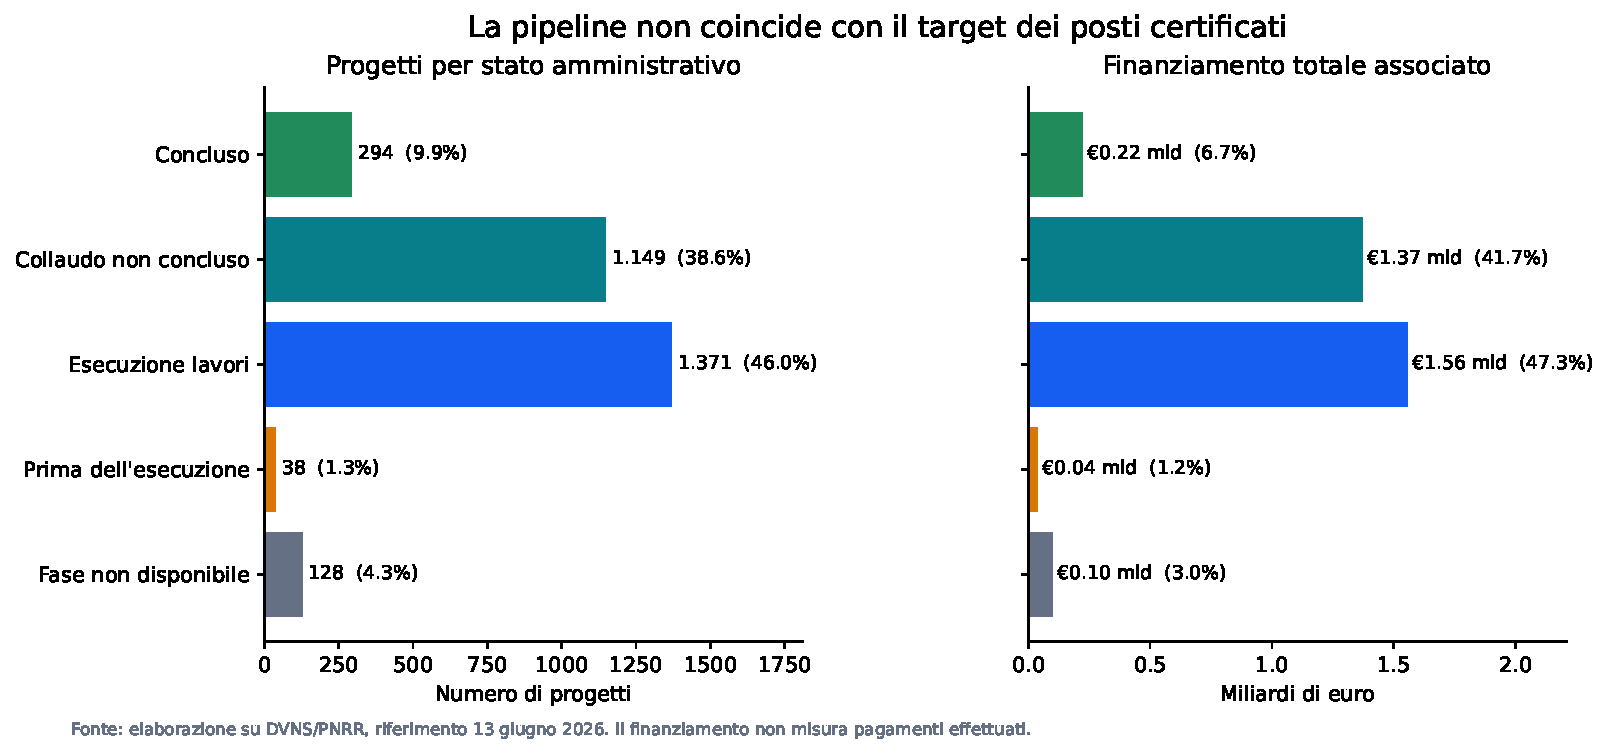
\includegraphics[width=\textwidth]{01_pipeline.pdf}
  \caption{Pipeline dei progetti e finanziamento associato}
  \label{fig:pipeline}
\end{figure}

\begin{table}[H]
\centering
\caption{Distribuzione della pipeline}
\label{tab:pipeline}
\begin{tabular}{lrrrr}
\toprule
Stato & Progetti & Quota & Mld \texteuro{} & Quota fondi \\
\midrule
Concluso & 294 & 9.9\% & 0.22 & 6.7\% \\
Collaudo non concluso & 1.149 & 38.6\% & 1.37 & 41.7\% \\
Esecuzione lavori & 1.371 & 46.0\% & 1.56 & 47.3\% \\
Prima dell'esecuzione & 38 & 1.3\% & 0.04 & 1.2\% \\
Fase non disponibile & 128 & 4.3\% & 0.10 & 3.0\% \\
\bottomrule
\end{tabular}

\end{table}

La distinzione tra collaudo e conclusione è sostanziale. Se li aggregassimo, diremmo che il 48,4\% è nella parte finale del ciclo. Se usassimo solo la conclusione, diremmo 9,9\%. Entrambi i numeri sono corretti per la loro definizione; nessuno dei due risponde alla domanda europea sui posti certificati.

\subsection{Una tensione tra perequazione finanziaria e maturità}

La quota di progetti almeno in collaudo varia dal 28,7\% in Calabria al 91,9\% in Trentino-Alto Adige; la Valle d'Aosta raggiunge il 75\%, ma su appena quattro progetti. Gli intervalli ricordano che confronti tra piccoli e grandi portafogli hanno precisione molto diversa.

\begin{figure}[H]
  \centering
  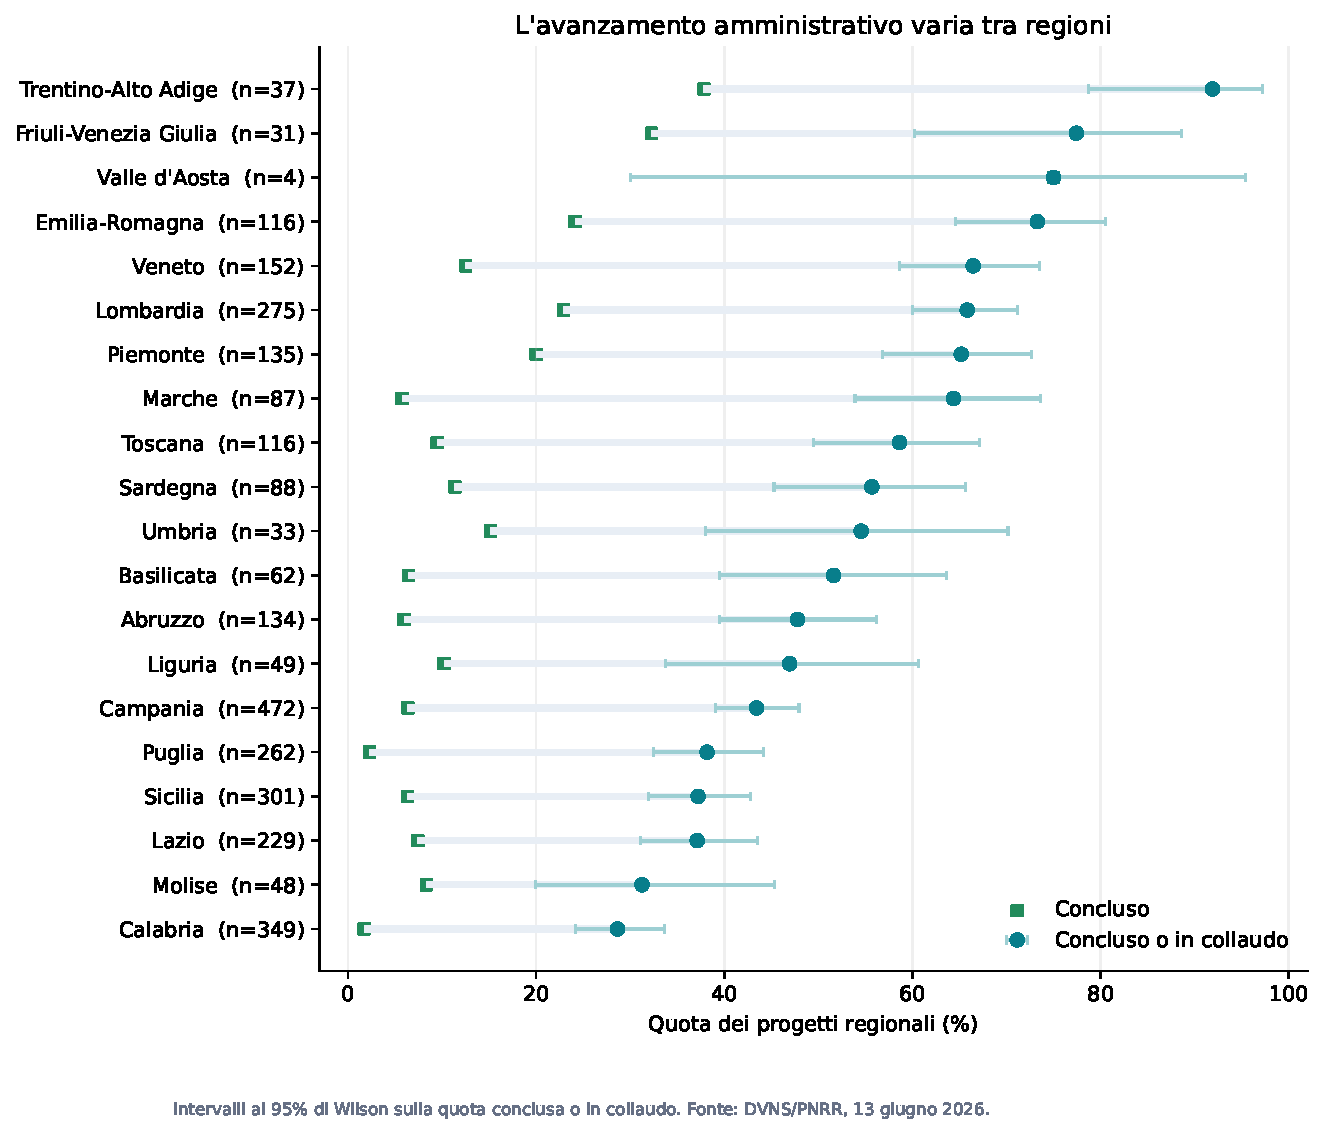
\includegraphics[width=\textwidth]{02_regioni_avanzamento.pdf}
  \caption{Conclusione e ingresso nel collaudo per regione}
  \label{fig:regions}
\end{figure}

Il risultato territoriale centrale emerge incrociando due assi. Dove la copertura Istat preesistente è minore, il finanziamento associato per bambino è tendenzialmente maggiore ($\rho=-0{,}58$, $p=0{,}007$). Questo è coerente con una logica perequativa dell'allocazione, pur senza provarne il meccanismo. Tuttavia, la quota di progetti conclusi o in collaudo è più alta nelle regioni con maggiore copertura ($\rho=0{,}59$, $p=0{,}007$); per i soli conclusi, $\rho=0{,}67$ ($p=0{,}001$).

\begin{figure}[H]
  \centering
  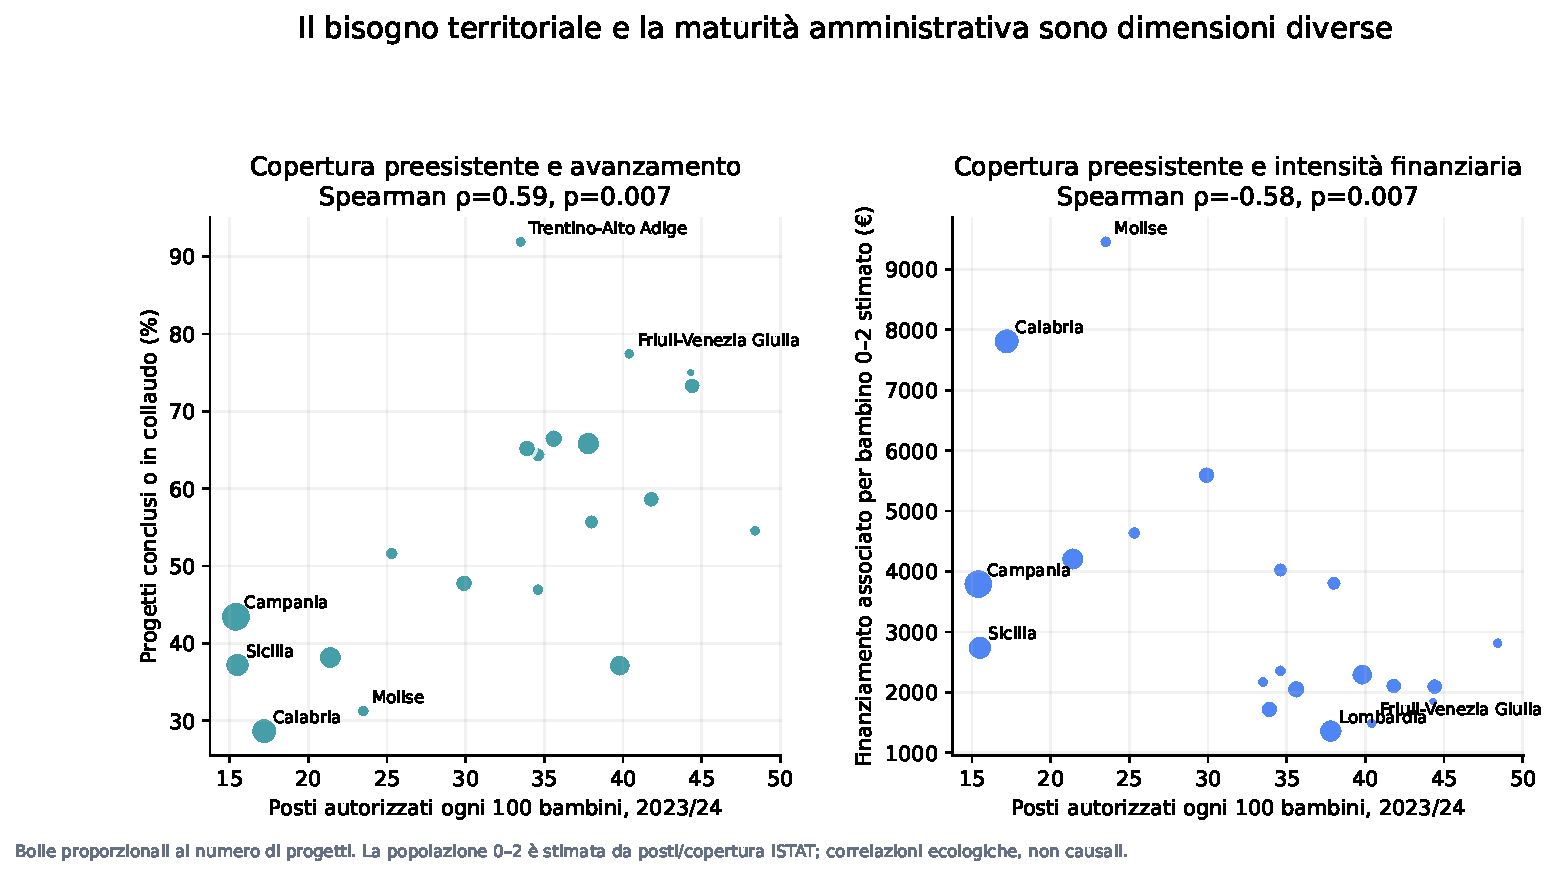
\includegraphics[width=\textwidth]{03_copertura_istat.pdf}
  \caption{Copertura preesistente, avanzamento e intensità finanziaria}
  \label{fig:coverage}
\end{figure}

Queste correlazioni non dicono che una bassa copertura causi ritardi. Le regioni differiscono per composizione dei progetti, data dei bandi, capacità dei comuni e altre variabili. Indicano però un rischio concreto di policy: la perequazione ex ante può essere attenuata da velocità di consegna diseguali. Il monitoraggio dovrebbe quindi misurare non soltanto dove sono allocate le risorse, ma se il divario di servizio si sta effettivamente chiudendo.

\subsection{L'impronta degli appalti}

Il campione contiene 13.715 procedure collegate; 2.816 progetti su 2.980 ne hanno almeno una. La mediana è quattro procedure per i conclusi e per quelli in esecuzione, cinque per i progetti in collaudo. Almeno una procedura classificata come lavori compare nel 97,6\% dei conclusi, nel 94,6\% dei progetti in collaudo e nel 94,1\% di quelli in esecuzione. Gli affidamenti diretti compaiono in oltre nove progetti maturi su dieci, spesso per una delle molte componenti del percorso.

\begin{figure}[H]
  \centering
  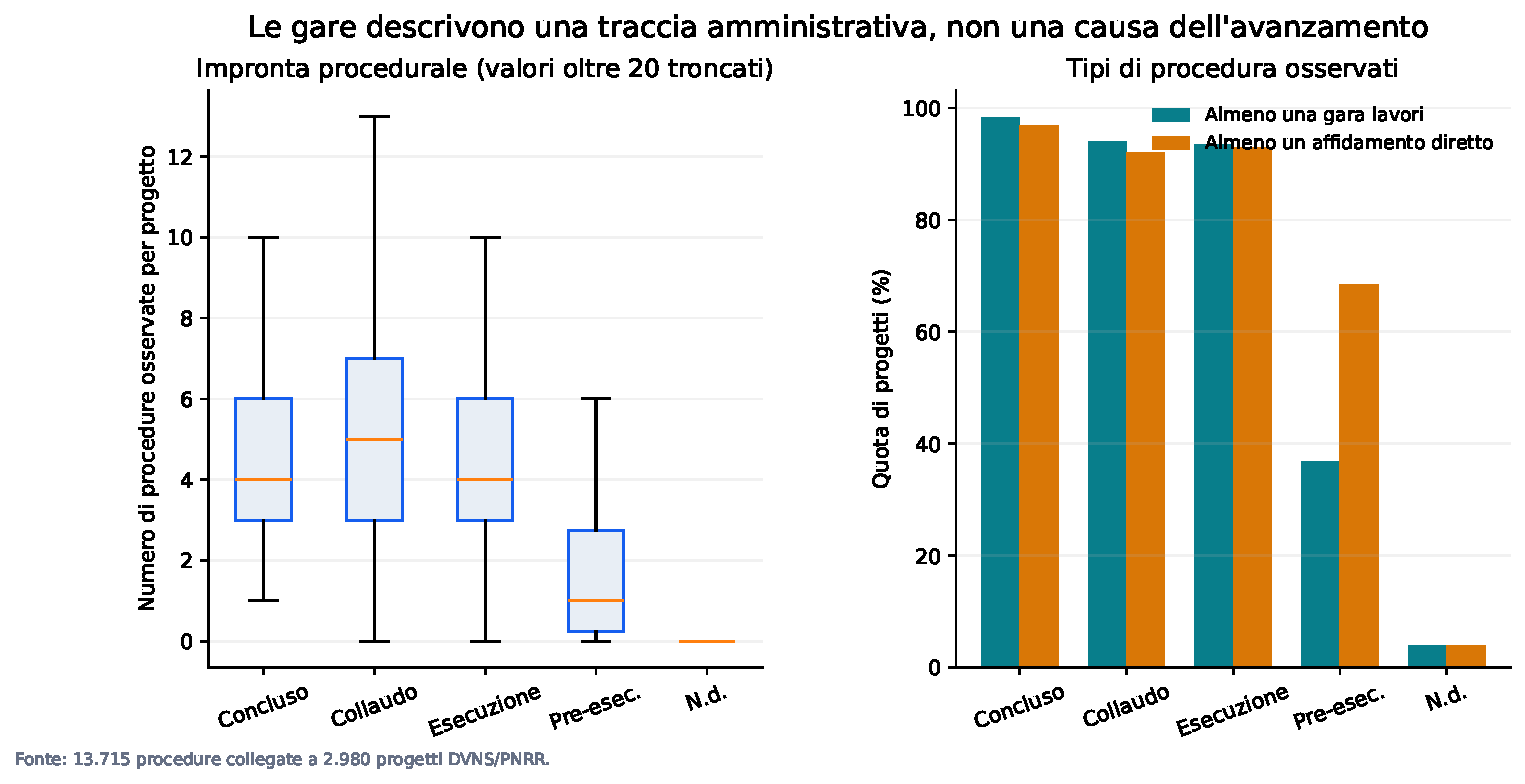
\includegraphics[width=\textwidth]{04_impronta_appalti.pdf}
  \caption{Numero e tipologia delle procedure lungo la pipeline}
  \label{fig:procurement}
\end{figure}

La figura non supporta l'equazione “più procedure = più ritardo” né la sua inversa. Le procedure si accumulano mentre il progetto avanza; un progetto complesso può averne di più; l'assenza di gare tra i record senza fase può riflettere incompletezza o uno stadio iniziale. L'impronta è utile per il triage e la tracciabilità, non per attribuire responsabilità causali.

\subsection{Associazioni condizionate}

La Figura~\ref{fig:models} riporta gli odds ratio dei modelli principali. Le associazioni più stabili sono:

\begin{itemize}
  \item \textbf{cronologia}: un anno di avvio più recente è associato a OR 0,47 per la conclusione e 0,63 per l'ingresso nel collaudo;
  \item \textbf{scala}: il raddoppio del finanziamento è associato a OR 0,42 e 0,79 rispettivamente;
  \item \textbf{tipo}: ampliamenti e ristrutturazioni/recuperi mostrano odds superiori alle nuove costruzioni; demolizione/ricostruzione non è distinguibile dalla categoria di riferimento;
  \item \textbf{territorio}: 10 punti in più di copertura regionale sono associati a OR 1,48 per la conclusione e 1,31 per l'ingresso nel collaudo;
  \item \textbf{procedure}: il raddoppio del numero di procedure più uno è associato a OR 1,21 per la conclusione e 1,16 per l'ingresso nel collaudo; il secondo intervallo include uno nella stima con clustering regionale.
\end{itemize}

\begin{figure}[H]
  \centering
  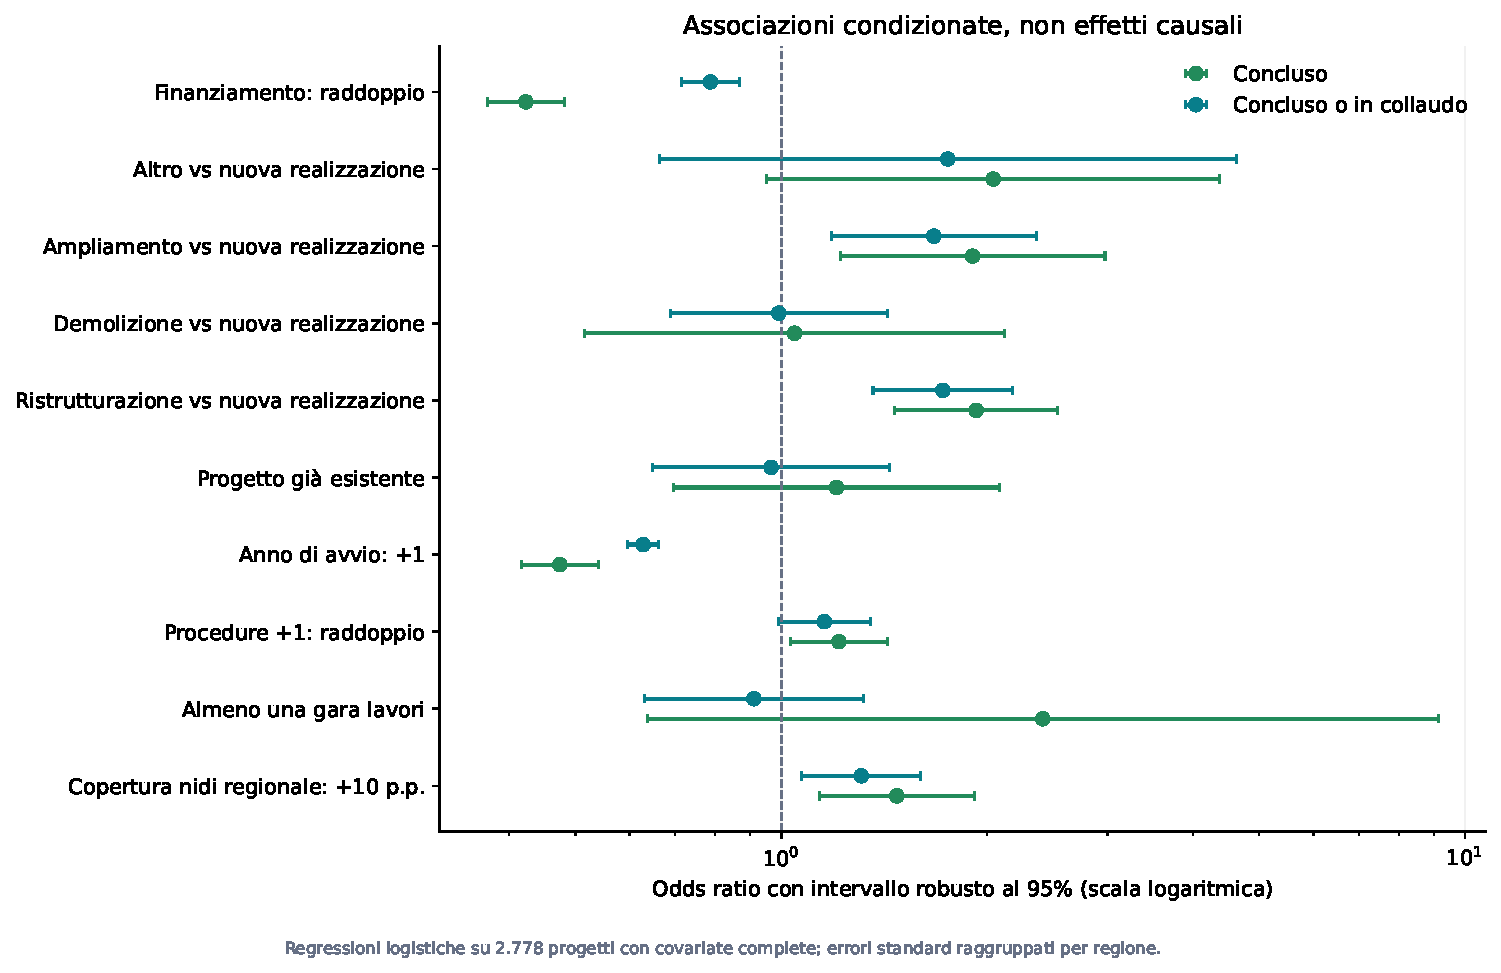
\includegraphics[width=\textwidth]{06_modelli.pdf}
  \caption{Regressioni logistiche della maturità amministrativa}
  \label{fig:models}
\end{figure}

\begin{table}[H]
\centering
\caption{Odds ratio dei modelli principali}
\label{tab:models}
\resizebox{\textwidth}{!}{\begin{tabular}{lcc}
\toprule
Covariata & Concluso & Concluso/collaudo \\
\midrule
Finanziamento (raddoppio) & 0.42*** [0.37; 0.48] & 0.79*** [0.71; 0.87] \\
Ampliamento & 1.90** [1.22; 2.97] & 1.67** [1.18; 2.36] \\
Demolizione/ricostruzione & 1.05 [0.52; 2.12] & 0.99 [0.69; 1.43] \\
Ristrutturazione/recupero & 1.93*** [1.47; 2.53] & 1.72*** [1.36; 2.18] \\
Progetto esistente & 1.20 [0.70; 2.09] & 0.97 [0.65; 1.44] \\
Anno di avvio (+1) & 0.47*** [0.42; 0.54] & 0.63*** [0.60; 0.66] \\
Procedure +1 (raddoppio) & 1.21* [1.03; 1.43] & 1.16 [0.99; 1.35] \\
Almeno una gara lavori & 2.41 [0.64; 9.14] & 0.91 [0.63; 1.32] \\
Copertura regionale (+10 p.p.) & 1.48** [1.14; 1.92] & 1.31** [1.07; 1.60] \\
\bottomrule
\end{tabular}
}
\begin{minipage}{0.96\textwidth}\footnotesize\color{dvnsgrey}
Intervalli al 95\% tra parentesi quadre. Errori standard raggruppati per regione. Categoria di riferimento: nuova realizzazione. * $p<0{,}05$; ** $p<0{,}01$; *** $p<0{,}001$. Gli odds ratio non sono variazioni di probabilità.
\end{minipage}
\end{table}

Questi risultati sono coerenti con un ciclo di produzione: opere iniziate prima, più piccole o basate su strutture da ampliare/recuperare sono più vicine alla consegna. Non dimostrano che ridurre la dimensione finanziaria o moltiplicare le procedure accelererebbe un progetto. In particolare, il modello non dispone di una misura diretta della qualità progettuale, della capacità dell'ente, dei contenziosi o degli shock di cantiere.

\section{Il dato più importante è quello che manca}

La base è tecnicamente ricca. Regione e finanziamento sono presenti per tutti i progetti; il 94,5\% ha almeno una procedura e il 93,2\% una data di avvio. Tra le procedure, importi, pubblicazione e tipo sono quasi sempre disponibili. La data di aggiudicazione scende al 69,7\%.

\begin{figure}[H]
  \centering
  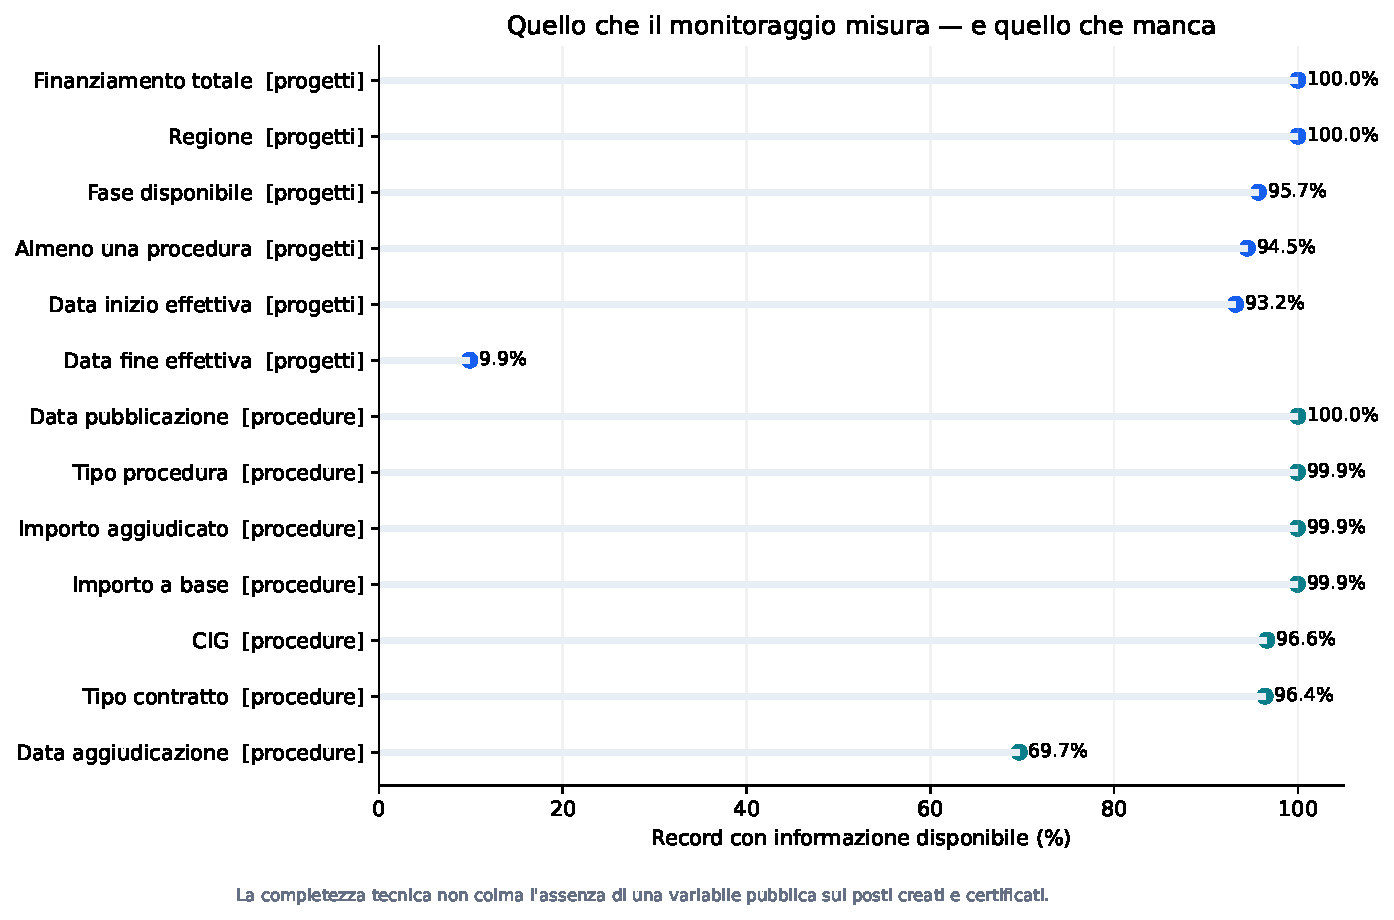
\includegraphics[width=0.92\textwidth]{05_completezza.pdf}
  \caption{Completezza dei campi osservati}
  \label{fig:completeness}
\end{figure}

La data di fine effettiva è presente esattamente per i 294 progetti conclusi. Non è quindi una validazione indipendente dello stato. Soprattutto, nessuno dei quattro asset integrati espone per CUP:

\begin{itemize}
  \item posti previsti, distinti tra nuovi, riqualificati, ampliati e cambio d'uso;
  \item posti coperti da un certificato di completamento e data del certificato;
  \item struttura fisica e identificativo del servizio che riceverà i posti;
  \item data di apertura, posti autorizzati, occupati e in lista d'attesa;
  \item personale necessario e personale effettivamente disponibile;
  \item uno storico versionato delle fasi e delle variazioni di importo.
\end{itemize}

Questa assenza cambia la domanda a cui l'open data può rispondere. Si può verificare che un progetto esista, dove sia localizzato, quanto finanziamento gli sia associato e quali procedure siano collegate. Non si può sommare un numero indipendentemente verificabile di posti certificati, né collegare gli euro all'apertura e all'utilizzo del servizio.

\section{Robustezza e limiti}

\subsection{Definizioni alternative}

I risultati descrittivi non dipendono da un'unica scelta di campione. Escludendo i 128 record con fase non disponibile, la quota almeno in collaudo sale dal 48,4\% al 50,6\%. Tra i 1.585 progetti avviati entro il 2023, il 17,0\% è concluso e il 61,6\% almeno in collaudo. Sull'intera misura 0--6, le quote sono 10,2\% e 50,1\%, vicine al campione principale.

\begin{table}[H]
\centering
\caption{Controlli descrittivi di sensibilità}
\label{tab:sensitivity}
\resizebox{0.92\textwidth}{!}{\begin{tabular}{lrlr}
\toprule
Campione & N & Esito & Quota \\
\midrule
Campione completo & 2.980 & Concluso & 9.9\% \\
Campione completo & 2.980 & Concluso o in collaudo & 48.4\% \\
Campione completo & 2.980 & Data fine effettiva presente & 9.9\% \\
Esclusa fase non disponibile & 2.852 & Concluso o in collaudo & 50.6\% \\
Avvio entro il 2023 & 1.585 & Concluso & 17.0\% \\
Avvio entro il 2023 & 1.585 & Concluso o in collaudo & 61.6\% \\
Intera misura 0--6 & 3.841 & Concluso & 10.2\% \\
Intera misura 0--6 & 3.841 & Concluso o in collaudo & 50.1\% \\
\bottomrule
\end{tabular}
}
\end{table}

I modelli con effetti fissi regionali mantengono il segno delle associazioni principali per anno, scala e tipologia. Non attribuiamo valore strutturale alle dimensioni esatte degli odds ratio: la selezione nei bandi, la revisione del PNRR e l'assenza di covariate comunali possono produrre confondimento residuo.

\subsection{Otto limiti da non perdere}

\begin{enumerate}
  \item \textbf{Snapshot, non pannello.} Osserviamo lo stato al 13 giugno 2026, non la traiettoria completa.
  \item \textbf{Stato amministrativo, non risultato fisico.} “Concluso” non è un certificato di posti.
  \item \textbf{Classificazione amministrativa.} Il filtro \texttt{ASILI NIDO} migliora la coerenza, ma non sostituisce la verifica del contenuto dell'opera.
  \item \textbf{Finanziamento, non pagamento.} Gli importi associati e di gara non sono erogazioni osservate.
  \item \textbf{Copertura regionale.} Il benchmark territoriale è aggregato e precedente; non descrive il bacino comunale di ogni progetto.
  \item \textbf{Endogeneità.} Data di avvio, numero di gare, scala e fase co-evolvono con complessità e capacità non osservate.
  \item \textbf{Complete cases.} Le regressioni escludono 202 progetti senza anno di avvio e altri casi senza covariate.
  \item \textbf{Data di riferimento.} Successivi aggiornamenti possono modificare lo stato; gli hash rendono questa versione replicabile, non eternamente attuale.
\end{enumerate}

\section{Implicazioni per la politica pubblica}

\subsection{Dalla dashboard di spesa a un registro di consegna}

Proponiamo un'estensione minima, pubblicabile senza dati personali:

\begin{enumerate}
  \item \textbf{chiave di risultato}: CUP, identificativo struttura e comune;
  \item \textbf{denominatore fisico}: posti previsti per tipo e fascia d'età;
  \item \textbf{verifica}: posti certificati, data e identificativo del certificato;
  \item \textbf{attivazione}: autorizzazione, data di apertura, posti attivi, occupati e lista d'attesa;
  \item \textbf{sostenibilità}: personale equivalente a tempo pieno previsto e disponibile, titolarità pubblica/privata, ore e mesi di servizio;
  \item \textbf{storia}: timestamp di ogni passaggio di fase, variazione finanziaria e revisione del target.
\end{enumerate}

Il registro dovrebbe essere versionato e interrogabile, con dizionario dei campi e hash di ogni rilascio. Il monitoraggio civico potrebbe allora riprodurre tre conti distinti: risorse assegnate, infrastrutture consegnate, servizio disponibile.

\subsection{Una lista di priorità derivata dai dati}

La fotografia suggerisce un ordine di attenzione, non una classifica di colpe.

\begin{itemize}
  \item \textbf{1.371 progetti in esecuzione}: richiedono monitoraggio di cantiere e delle date previste/effettive, non nuove statistiche sulle sole gare.
  \item \textbf{1.149 in collaudo}: richiedono visibilità su certificati, autorizzazioni e passaggio all'apertura; è qui che la distinzione tra opera e servizio diventa decisiva.
  \item \textbf{128 senza fase}: richiedono bonifica e responsabilità sulla qualità informativa.
  \item \textbf{territori con bassa copertura e bassa maturità}: richiedono assistenza tecnica mirata e un controllo sugli esiti, perché il maggior finanziamento per bambino non garantisce di per sé la riduzione del divario.
\end{itemize}

Non segue dai nostri dati che si debbano ridurre controlli, eliminare gare o premiare una regione. Segue che lo strumento di gestione deve essere calibrato sulla fase: progettazione, cantiere, collaudo e apertura sono colli di bottiglia diversi.

\section{Conclusioni}

Alla vigilia della scadenza osservata, il PNRR per gli asili nido presenta una pipeline divisa: quasi metà dei progetti ha raggiunto almeno il collaudo, ma solo uno su dieci è registrato come concluso. L'allocazione appare più intensa dove la dotazione iniziale è minore; l'avanzamento è invece maggiore nei territori già più coperti. È il risultato più importante dello studio: una politica disegnata per ridurre divari può incontrare un rischio di consegna che riproduce parte di quei divari.

La cronologia, la scala e il tipo di opera spiegano associazioni più nette della semplice presenza di gare. Questo non assolve né accusa alcun attore: indica che l'unità di analisi utile è il percorso completo del progetto. Il dibattito centrato soltanto su assegnazioni o procedure perde il passaggio tra cantiere, certificato e servizio.

Il limite dei dati è anche una proposta di ricerca. Pubblicare posti previsti e certificati per CUP, insieme a uno storico delle fasi e a indicatori di apertura e utilizzo, renderebbe possibile un vero studio di efficacia: non “quanto abbiamo finanziato?”, ma “dove sono diventati disponibili posti, per chi e con quale capacità operativa?”. Fino ad allora, il giudizio corretto è più modesto e più utile: sappiamo misurare una pipeline amministrativa sotto pressione; non sappiamo ancora verificare pubblicamente il risultato finale che la politica promette.

\clearpage
\appendix

\section{Risultati regionali completi}
\label{app:regions}

La Tabella~\ref{tab:regionsfull} riporta numerosità, quota conclusa, quota almeno in collaudo, copertura Istat e finanziamento associato per popolazione 0--2 stimata. I valori non sono graduatorie di performance: differiscono per dimensione del portafoglio, composizione e storia dei bandi.

\begin{table}[H]
\centering
\caption{Risultati per regione, campione ASILI NIDO}
\label{tab:regionsfull}
\resizebox{\textwidth}{!}{\begin{tabular}{lrrrrr}
\toprule
Regione & N & Conclusi & Conclusi/collaudo & Copertura & \texteuro{}/bambino \\
\midrule
Abruzzo & 134 & 6.0\% & 47.8\% & 29.9 & 5593 \\
Basilicata & 62 & 6.5\% & 51.6\% & 25.3 & 4637 \\
Calabria & 349 & 1.7\% & 28.7\% & 17.2 & 7809 \\
Campania & 472 & 6.4\% & 43.4\% & 15.4 & 3791 \\
Emilia-Romagna & 116 & 24.1\% & 73.3\% & 44.4 & 2094 \\
Friuli-Venezia Giulia & 31 & 32.3\% & 77.4\% & 40.4 & 1488 \\
Lazio & 229 & 7.4\% & 37.1\% & 39.8 & 2292 \\
Liguria & 49 & 10.2\% & 46.9\% & 34.6 & 2354 \\
Lombardia & 275 & 22.9\% & 65.8\% & 37.8 & 1358 \\
Marche & 87 & 5.7\% & 64.4\% & 34.6 & 4025 \\
Molise & 48 & 8.3\% & 31.2\% & 23.5 & 9456 \\
Piemonte & 135 & 20.0\% & 65.2\% & 33.9 & 1717 \\
Puglia & 262 & 2.3\% & 38.2\% & 21.4 & 4207 \\
Sardegna & 88 & 11.4\% & 55.7\% & 38.0 & 3806 \\
Sicilia & 301 & 6.3\% & 37.2\% & 15.5 & 2737 \\
Toscana & 116 & 9.5\% & 58.6\% & 41.8 & 2106 \\
Trentino-Alto Adige & 37 & 37.8\% & 91.9\% & 33.5 & 2170 \\
Umbria & 33 & 15.2\% & 54.5\% & 48.4 & 2813 \\
Valle d'Aosta & 4 & 75.0\% & 75.0\% & 44.3 & 1851 \\
Veneto & 152 & 12.5\% & 66.4\% & 35.6 & 2050 \\
\bottomrule
\end{tabular}
}
\begin{minipage}{0.93\linewidth}\footnotesize\color{dvnsgrey}
Copertura: posti autorizzati per 100 bambini 0--2, Istat 2023/24. €/bambino: finanziamento totale associato diviso per la popolazione 0--2 stimata da posti/copertura. Non è spesa erogata.
\end{minipage}
\end{table}

\section{Dizionario minimo delle variabili}

\begin{longtable}{p{0.25\textwidth}p{0.67\textwidth}}
\toprule
\textbf{Variabile} & \textbf{Definizione} \\
\midrule
\endfirsthead
\toprule
\textbf{Variabile} & \textbf{Definizione} \\
\midrule
\endhead
CUP & Codice unico di progetto, chiave pubblica di progetto. \\
Categoria & Categoria amministrativa del progetto; il campione principale richiede il valore \texttt{ASILI NIDO}. \\
Concluso & Avanzamento pari a \texttt{Concluso}. \\
Concluso/collaudo & Concluso oppure fase contenente \texttt{COLLAUDO}. \\
Finanziamento totale & Somma delle componenti di finanziamento associate al progetto nella fonte; non pagamento. \\
Finanziamento PNRR & Quota PNRR associata; non pagamento. \\
Anno di avvio & Anno della data di inizio effettiva; mancante per 202 progetti del campione. \\
Tipo progetto & Riclassificazione deterministica di nuova realizzazione, ampliamento, recupero/ristrutturazione, demolizione/ricostruzione, altro. \\
Numero procedure & Conteggio delle righe gara collegate al CUP; non numero di lavori distinti. \\
Gara lavori & Almeno una procedura con tipo contratto contenente \texttt{LAVORI}. \\
Copertura regionale & Posti autorizzati per 100 bambini 0--2, Istat 2023/24. \\
\bottomrule
\end{longtable}

\section{Completezza dei campi}

\begin{table}[H]
\centering
\caption{Disponibilità delle informazioni usate}
\resizebox{0.82\textwidth}{!}{\begin{tabular}{llr}
\toprule
Livello & Campo & Disponibile \\
\midrule
Procedure & Data aggiudicazione & 69.7\% \\
Procedure & Tipo contratto & 96.4\% \\
Procedure & CIG & 96.6\% \\
Procedure & Importo a base & 99.9\% \\
Procedure & Importo aggiudicato & 99.9\% \\
Procedure & Tipo procedura & 99.9\% \\
Procedure & Data pubblicazione & 100.0\% \\
Progetti & Data fine effettiva & 9.9\% \\
Progetti & Data inizio effettiva & 93.2\% \\
Progetti & Almeno una procedura & 94.5\% \\
Progetti & Fase disponibile & 95.7\% \\
Progetti & Regione & 100.0\% \\
Progetti & Finanziamento totale & 100.0\% \\
\bottomrule
\end{tabular}
}
\end{table}

Le percentuali pari a 100,0\% possono essere leggermente inferiori a uno prima dell'arrotondamento. La completezza è calcolata sul campione principale e sulle 13.715 procedure a esso collegate.

\section{Riproducibilità e integrità}
\label{app:repro}

\subsection{Query MCP}

La verifica compatta usa il seguente invito JSON-RPC all'endpoint \url{https://www.dovevannoinostrisoldi.com/api/mcp}:

\begin{verbatim}
{
  "jsonrpc": "2.0",
  "id": 1,
  "method": "tools/call",
  "params": {
    "name": "query_dataset",
    "arguments": {"dataset": "pnrr_asili", "limit": 1}
  }
}
\end{verbatim}

Il controllo richiede 3.841 progetti, 18.851 procedure e 5.061.145.343,73 euro di finanziamento totale associato per l'intera misura.

\subsection{Hash SHA-256}

\begin{table}[H]
\centering
\scriptsize
\caption{Impronte delle fonti e dello snapshot analizzato}
\begin{tabular}{p{0.18\textwidth}p{0.72\textwidth}}
\toprule
Asset & SHA-256 \\
\midrule
Progetti & \texttt{1b1913c5b71df0794450522e1563b6d5b637356279779f6134b3af98d90df74d} \\
Gare & \texttt{1154c0796958cb36a7b64addb850eb2812b118ba8a5f8a0b22c32f56be7f8525} \\
Localizzazioni & \texttt{0fae9b0252b7e0949d0c11d374c3113178c096da1077462810971a0eac07bbcd} \\
Aggiudicatari & \texttt{0b2a2956df880c93e75f60026a0e53ebb489a7d1b66f1a7b4fd304d077302818} \\
Snapshot integrato & \texttt{5693cfe012b8de38c065852f0d040e54fda982ca98704e7faaf3a2566c3e0da2} \\
\bottomrule
\end{tabular}
\end{table}

\subsection{Pipeline di riproduzione}

Lo script \texttt{scripts/analyze.py}:

\begin{enumerate}
  \item verifica l'hash dello snapshot e i totali contro \texttt{data/mcp\_pnrr\_manifest.json};
  \item estrae un record per CUP senza nomi o codici fiscali degli aggiudicatari;
  \item applica il filtro \texttt{ASILI NIDO} e genera i due esiti;
  \item unisce la sola copertura regionale Istat;
  \item produce CSV analitici, tabelle LaTeX, figure PDF/PNG e un riepilogo JSON;
  \item stima i modelli con versioni software fissate in \texttt{requirements.txt}.
\end{enumerate}

Ogni numero nel testo deriva da questi artefatti. Il manifest conserva anche data di interrogazione, copertura e avvertenze interpretative. Nessuna credenziale è necessaria e l'MCP è in sola lettura.

\clearpage
\begin{thebibliography}{99}

\bibitem[Bulman(2021)]{bulman2021}
Bulman, T. (2021).
\newblock Strengthening Italy's public sector effectiveness.
\newblock \emph{OECD Economics Department Working Papers}, 1690.
\newblock \url{https://doi.org/10.1787/823cad2a-en}.

\bibitem[Carta and Rizzica(2018)]{carta2018}
Carta, F. and Rizzica, L. (2018).
\newblock Early kindergarten, maternal labor supply and children's outcomes: Evidence from Italy.
\newblock \emph{Journal of Public Economics}, 158, 79--102.
\newblock \url{https://doi.org/10.1016/j.jpubeco.2017.12.012}.

\bibitem[Cerqua et~al.(2025)Cerqua, Giannantoni, Zampollo, and Mazziotta]{cerqua2025}
Cerqua, A., Giannantoni, C., Zampollo, F. and Mazziotta, M. (2025).
\newblock The Municipal Administration Quality Index: The Italian Case.
\newblock \emph{Social Indicators Research}, 177(1), 345--378.
\newblock \url{https://doi.org/10.1007/s11205-024-03511-8}.

\bibitem[Del Monte et~al.(2025)Del Monte, De Iudicibus, Moccia, and Pennacchio]{delmonte2025}
Del Monte, A., De Iudicibus, A., Moccia, S. and Pennacchio, L. (2025).
\newblock Administrative capacity and speed of public spending.
\newblock \emph{Regional Studies}, 59(1).
\newblock \url{https://doi.org/10.1080/00343404.2025.2552865}.

\bibitem[DoveVannoINostriSoldi(2026)]{dvns2026}
DoveVannoINostriSoldi (2026).
\newblock Dataset integrato PNRR: asili nido e servizi per la prima infanzia.
\newblock Dataset \texttt{pnrr\_asili}, riferimento 13 giugno 2026.
\newblock \url{https://www.dovevannoinostrisoldi.com/mcp}.

\bibitem[European Commission(2026)]{ec2026target}
European Commission (2026).
\newblock Annex to the Proposal for a Council Implementing Decision amending the approval of Italy's recovery and resilience plan.
\newblock COM(2026) 114 final, target M4C1-18.
\newblock \url{https://eur-lex.europa.eu/legal-content/EN/ALL/?uri=CELEX:52026PC0114}.

\bibitem[Fantozzi(2025)]{upb2025}
Fantozzi, R. (2025).
\newblock Piano asili nido e scuole dell'infanzia: stato di attuazione e obiettivi del PNRR e del PSB.
\newblock \emph{Ufficio parlamentare di bilancio, Focus tematico n. 1}.
\newblock \url{https://www.upbilancio.it/it/piano-asili-nido-e-scuole-dellinfanzia-stato-di-attuazione-e-obiettivi-del-pnrr-e-del-psb/}.

\bibitem[Istat(2026)]{istat2026}
Istituto Nazionale di Statistica (2026).
\newblock Offerta di nidi e servizi integrativi per la prima infanzia: anno educativo 2023--2024.
\newblock \url{https://www.istat.it/comunicato-stampa/offerta-di-nidi-e-servizi-integrativi-per-la-prima-infanzia-anno-educativo-2023-2024/}.

\bibitem[Lippi and Terlizzi(2023)]{lippi2023}
Lippi, A. and Terlizzi, A. (2023).
\newblock The marble cake of social services in Italy and Spain: Policy capacity, social investment, and the national recovery and resilience plans.
\newblock \emph{European Journal of Social Security}, 25(2).
\newblock \url{https://doi.org/10.1177/13882627231169266}.

\bibitem[Presidenza del Consiglio dei Ministri(2026)]{italiadomani2026}
Presidenza del Consiglio dei Ministri (2026).
\newblock Italia Domani: catalogo Open Data del PNRR.
\newblock Dataset Progetti, Gare, Localizzazioni e Aggiudicatari, CC BY 4.0.
\newblock \url{https://www.italiadomani.gov.it/content/sogei-ng/it/it/catalogo-open-data.html}.

\bibitem[Torrini(2025)]{torrini2025}
Torrini, R. (2025).
\newblock Audizione nell'ambito dell'indagine conoscitiva sui livelli essenziali delle prestazioni.
\newblock Banca d'Italia.
\newblock \url{https://www.bancaditalia.it/pubblicazioni/interventi-vari/int-var-2025/Audizione_Torrini_18marzo2025.pdf}.

\bibitem[Zanardi and Fantozzi(2026)]{zanardi2026}
Zanardi, A. and Fantozzi, R. (2026).
\newblock Correcting public service misallocation through intermunicipal mobility: evidence from Italy's RRF childcare program.
\newblock Research Square preprint.
\newblock \url{https://doi.org/10.21203/rs.3.rs-10219436/v1}.

\end{thebibliography}

\end{document}
